% IVP Group 19 project poster (A1 portrait). Build: run pdflatex Group19_Project_Poster.tex three times (equal-height rows use the .aux file).
\documentclass{article}
\usepackage[paperwidth=594mm,paperheight=841mm,margin=14mm,bottom=22mm]{geometry}
\usepackage[T1]{fontenc}
\usepackage[scaled]{helvet}
\renewcommand\familydefault{\sfdefault}
\usepackage{anyfontsize}
\usepackage{amsmath,amssymb}
\usepackage{graphicx}
\usepackage{xcolor}
\usepackage{enumitem}
\usepackage{booktabs}
\usepackage{eso-pic}
\usepackage[most]{tcolorbox}
\usepackage{tikz}
\usetikzlibrary{arrows.meta,positioning}
\usepackage{pgfplots}
\pgfplotsset{compat=1.17}

% ---- colour theme modelled on the example conference posters ----
\definecolor{bgtop}{HTML}{3EBDE8}   % saturated cyan background
\definecolor{bgbot}{HTML}{9EDDF3}
\definecolor{hdrL}{HTML}{16297A}    % dark-blue section bars
\definecolor{hdrR}{HTML}{2E56C8}
\definecolor{navy}{HTML}{1A2F86}
\definecolor{titleblue}{HTML}{1B3FA0}
\definecolor{panel}{HTML}{F4FBFE}
\definecolor{soft}{HTML}{E3F4FB}
\definecolor{accent}{HTML}{0A7FB8}
\definecolor{refc}{HTML}{8FB8DE}
\definecolor{impc}{HTML}{1A2F86}
\pagestyle{empty}
\setlength{\parindent}{0pt}
\AddToShipoutPictureBG{\AtPageLowerLeft{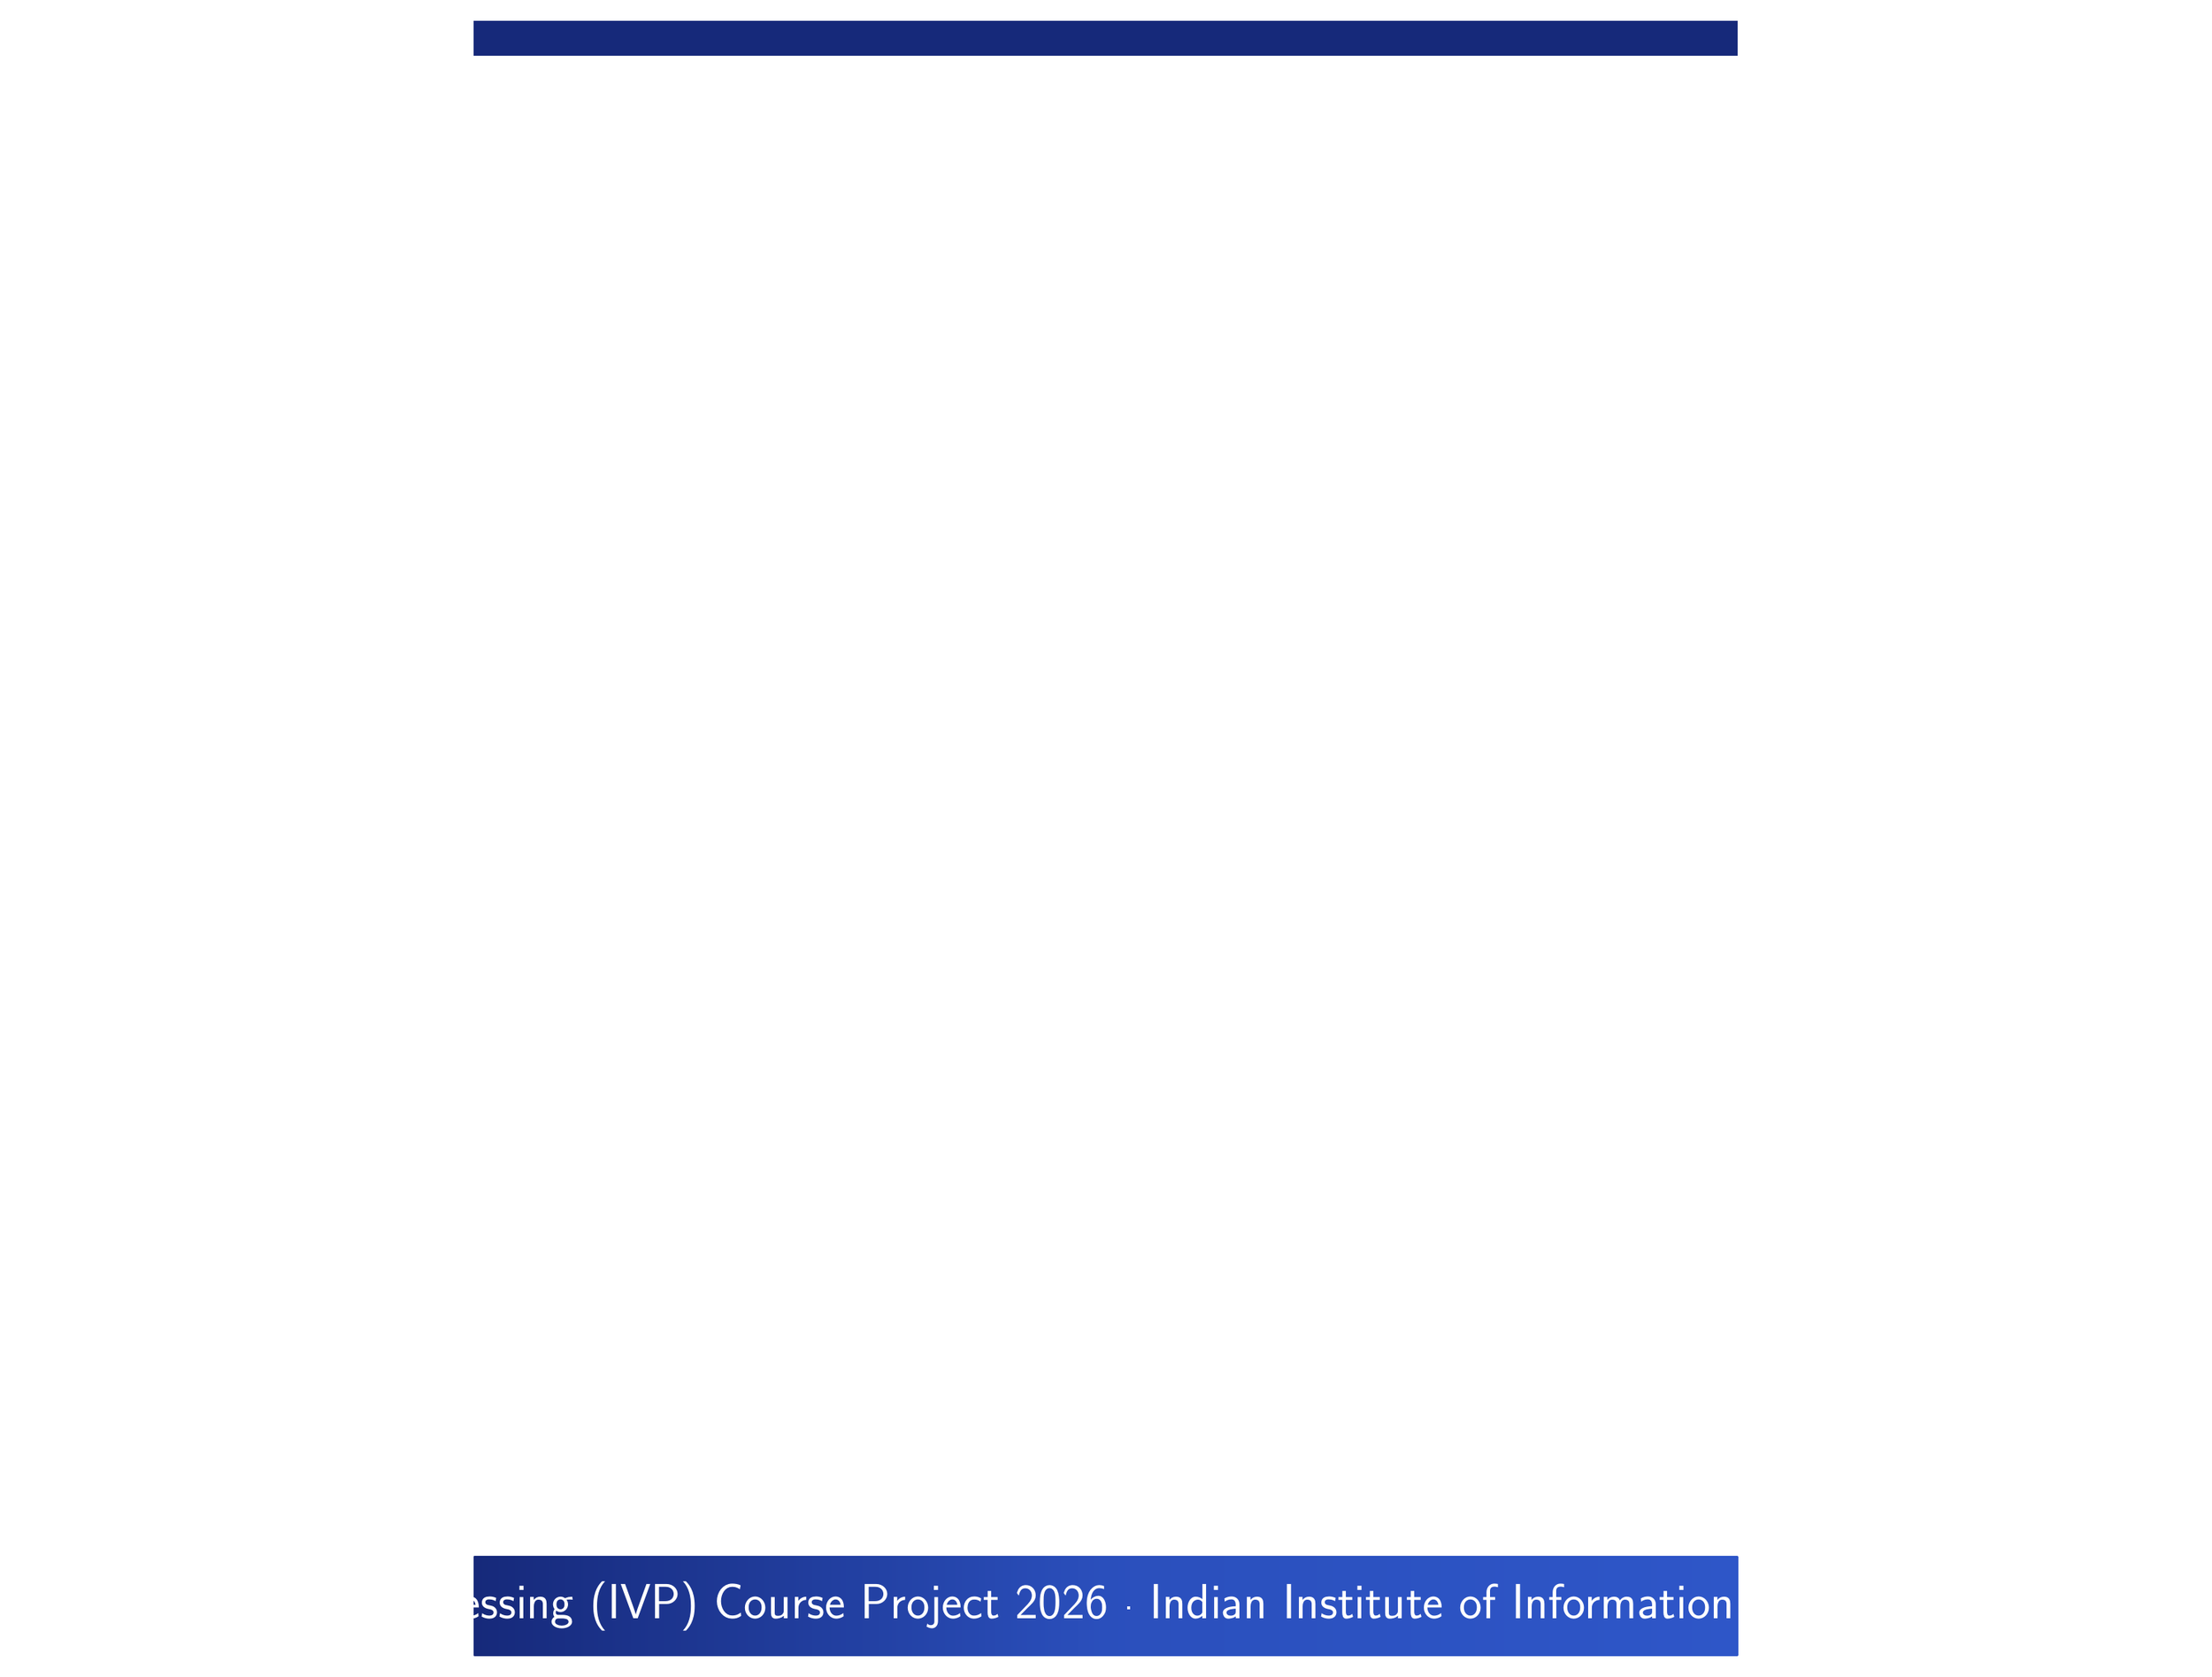
\begin{tikzpicture}
  \fill[white] (0,0) rectangle (\paperwidth,\paperheight);
  \shade[left color=hdrL,right color=hdrR,middle color=hdrR!85!hdrL] (0,0) rectangle (\paperwidth,17mm);
  \node[text=white,font=\fontsize{24}{28}\selectfont] at (0.5\paperwidth,8.5mm) {Image and Video Processing (IVP) Course Project 2026 \textperiodcentered{} Indian Institute of Information Technology, Allahabad};
  \fill[hdrL] (0,\paperheight-6mm) rectangle (\paperwidth,\paperheight);
\end{tikzpicture}}}

\newcommand\body{\fontsize{18}{22.5}\selectfont}
\newcommand\smalltext{\fontsize{15}{18.5}\selectfont}
\setlist{leftmargin=1.1em,itemsep=2pt,topsep=2pt,parsep=0pt}
\setlist[itemize]{label=\textcolor{navy}{\small$\blacktriangleright$}}

\newtcolorbox{psec}[2][]{enhanced,colback=panel,colframe=hdrL,boxrule=1.2pt,arc=2.5mm,
  title={#2},fonttitle=\bfseries\fontsize{30}{34}\selectfont,coltitle=white,
  title style={fill=hdrL},
  halign title=center,toptitle=2mm,bottomtitle=2mm,left=7mm,right=7mm,top=4mm,bottom=4mm,
  before skip=0pt,after skip=4mm,fontupper=\body,#1}

\tikzset{blk/.style={draw=navy,line width=1.1pt,rounded corners=3pt,align=center,fill=white,
  font=\fontsize{14}{17}\selectfont,minimum height=18mm,inner sep=3pt,
  execute at begin node={\hyphenpenalty=10000\exhyphenpenalty=10000}},
  hl/.style={blk,fill=soft},
  arr/.style={-{Stealth[length=8pt]},line width=1.8pt,draw=navy}}

\begin{document}

% ---------------- Header (as in the example posters: area line, title, authors, affiliation) ----------------
{\fontsize{26}{30}\selectfont\color{hdrL}\hfill Thematic Area -- Image and Video Processing\hfill\llap{\bfseries IVP Group 19}}\\[3mm]
\begin{center}
{\fontsize{62}{71}\selectfont\bfseries\color{titleblue}Multi-View Human Action Recognition:\\[2mm]
From TSN--GRU to an Attention-Based Architecture}\\[5mm]
{\fontsize{29}{35}\selectfont\color{black}Vichanshu Raj, Satwik Santosh, Vishwas Pahwa, Sudhanshu,\\[1mm]
Kyan Mahajan, Saumya Sood and Akshat Parmar}\\[4mm]
{\fontsize{25}{30}\selectfont\itshape\color{black}Indian Institute of Information Technology, Allahabad, Prayagraj, India}
\end{center}
\vspace{-2mm}

% ---------------- Abstract | Objectives ----------------
\begin{tcbraster}[raster columns=2,raster equal height=rows,raster column skip=8mm,raster after skip=4mm]
\begin{psec}[after skip=0pt]{Abstract}
Recognizing the same action from cameras at different viewpoints is hard because appearance, occlusion and motion direction change with the view. Building on the multi-branch Temporal Segment Network with GRU consensus of Bui and Nguyen~[1], with DVANet~[2] as the view-disentanglement reference, we study cross-view action recognition on the NW-UCLA RGB benchmark~[3]. The final ResNet-18 and temporal Transformer model reaches \textbf{94.2\%} cross-subject accuracy (macro-F1 0.88) and \textbf{88.97\%} on unseen camera 3 (macro-F1 0.83). The other cross-view splits score 81.3\% onto camera 1 and 83.4\% onto camera 2.
\end{psec}
\begin{psec}[after skip=0pt]{Objectives}
\begin{itemize}
\item Implement the multi-branch TSN~[4]\,+\,GRU~[5] pipeline of the base paper~[1] on NW-UCLA RGB video~[3] under cross-subject and cross-view protocols.
\item Add clip-consistent data augmentation (one flip and one brightness/contrast setting per clip) that preserves the order of motion.
\item Design a lighter improved architecture that classifies a single unseen camera view without duplicating it into two branches.
\item Evaluate with accuracy, macro precision, recall and F1 and confusion matrices, and deliver a working video-classification demo.
\end{itemize}
\end{psec}
\end{tcbraster}

% ---------------- Introduction | Methodology ----------------
\begin{tcbraster}[raster columns=2,raster equal height=rows,raster column skip=8mm,raster after skip=4mm]
\begin{psec}[after skip=0pt]{Introduction}
\begin{itemize}
\item Human action recognition gives one label to a video clip. Across cameras the same action looks different because of occlusion, perspective and motion direction, so multi-view methods fuse or exchange information between camera branches~[6],~[7].
\item TSN~[4] samples sparse snippets over the whole clip. The base paper~[1] adds per-view branches and a GRU~[5] that keeps snippet order: 93.81\% cross-subject and 84.4\% mean cross-view on NW-UCLA.
\item View-invariant methods use contrastive objectives~[8]. DVANet~[2] separates action and view features with transformer queries (94.4\% / 96.5\%), but needs view labels, triplets and a 3D encoder.
\item \textbf{Gap:} a lightweight model that keeps temporal order and aligns views without view labels.
\end{itemize}
\vspace{3mm}
\centering\includegraphics[width=0.8\linewidth]{../05_Summary_Paper/sample_segments.png}\\[1mm]
{\smalltext Fig.~1. Ordered segment frames of an NW-UCLA clip (pick up with one hand)~[3].}\\[3mm]
\begin{tcolorbox}[colback=white,colframe=accent,boxrule=1.1pt,arc=2mm,left=5mm,right=5mm,top=2mm,bottom=2mm,fontupper=\smalltext]
\textbf{Dataset: Northwestern-UCLA RGB~[3].} 1,475 videos, 10 actions, 10 subjects, 3 Kinect views, 418 complete three-view groups. Cross-view: train on two cameras, test on the third.
\end{tcolorbox}
\end{psec}
\begin{psec}[after skip=0pt]{Methodology}
\textbf{\color{navy}Stage 1: TSN--GRU~[1] with clip-consistent augmentation}\\[3mm]
\centering
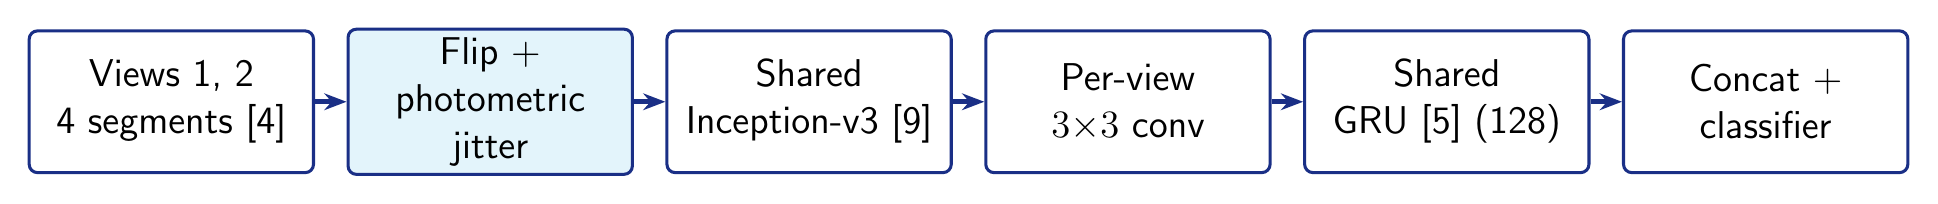
\begin{tikzpicture}[node distance=4mm]
\node[blk,text width=34mm] (a) {Views 1, 2\\4 segments~[4]};
\node[hl,text width=34mm,right=of a] (b) {Flip +\\photometric jitter};
\node[blk,text width=34mm,right=of b] (c) {Shared\\Inception-v3~[9]};
\node[blk,text width=34mm,right=of c] (d) {Per-view\\$3{\times}3$ conv};
\node[blk,text width=34mm,right=of d] (e) {Shared\\GRU~[5] (128)};
\node[blk,text width=34mm,right=of e] (f) {Concat +\\classifier};
\draw[arr] (a)--(b); \draw[arr] (b)--(c); \draw[arr] (c)--(d); \draw[arr] (d)--(e); \draw[arr] (e)--(f);
\end{tikzpicture}\\[2mm]
\raggedright
{\smalltext Flip ($p=0.5$) and contrast $[0.9,1.1]$ / brightness $[-8,8]$ ($p=0.5$), drawn once per clip so all frames change together.}\\[5mm]
\textbf{\color{navy}Stage 2: Improved architecture (proposed)}\\[3mm]
\centering
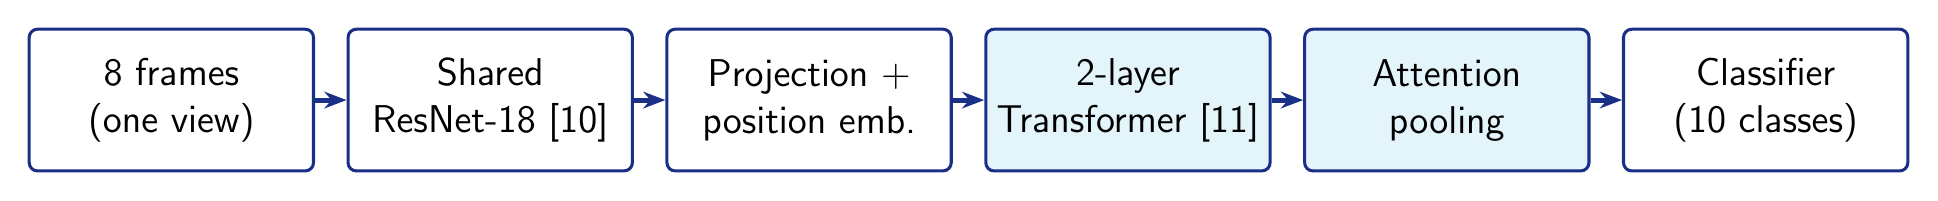
\begin{tikzpicture}[node distance=4mm]
\node[blk,text width=34mm] (a) {8 frames\\(one view)};
\node[blk,text width=34mm,right=of a] (b) {Shared\\ResNet-18~[10]};
\node[blk,text width=34mm,right=of b] (c) {Projection +\\position emb.};
\node[hl,text width=34mm,right=of c] (d) {2-layer\\Transformer~[11]};
\node[hl,text width=34mm,right=of d] (e) {Attention\\pooling};
\node[blk,text width=34mm,right=of e] (f) {Classifier\\(10 classes)};
\draw[arr] (a)--(b); \draw[arr] (b)--(c); \draw[arr] (c)--(d); \draw[arr] (d)--(e); \draw[arr] (e)--(f);
\end{tikzpicture}\\[2mm]
\raggedright
{\smalltext Views 1 and 2 of the same event share all weights and are tied by a paired-view cosine loss on their embeddings $e_v$:
\[\mathcal L=\tfrac12\textstyle\sum_{v=1}^{2}\mathcal L_{ce}(\hat y_v,y)+0.1\,\bigl(1-\cos(e_1,e_2)\bigr)\]
AdamW~[12] ($3{\times}10^{-4}$; backbone $3{\times}10^{-5}$), cosine schedule~[13], label smoothing 0.05~[9], batch 2, seed 42, implemented in PyTorch~[14]. The final scores are the four-protocol evaluation in Table~1. At test time one clip of the unseen camera is classified directly.}
\end{psec}
\end{tcbraster}

% ---------------- Results and Discussion ----------------
\begin{psec}{Results and Discussion}
\begin{minipage}[t]{0.58\linewidth}
\vspace{0pt}\centering
{\smalltext\textbf{Table 1.} Final accuracy (\%) and macro-F1 on NW-UCLA RGB~[3].}\\[2mm]
{\fontsize{16}{20.5}\selectfont
\renewcommand{\arraystretch}{1.18}
\begin{tabular}{@{}lccc@{}}
\toprule
Experiment & Accuracy & Macro-F1 & Base paper~[1]\\\midrule
Cross-subject & \textbf{94.2} & 0.88 & 93.81\\
Cross-view $\{2,3\}\to1$ & \textbf{81.3} & 0.79 & 82.58\\
Cross-view $\{1,3\}\to2$ & \textbf{83.4} & 0.81 & 81.00\\
Cross-view $\{1,2\}\to3$ & \textbf{88.97} & 0.83 & 89.76\\\bottomrule
\end{tabular}}
\end{minipage}\hfill
\begin{minipage}[t]{0.39\linewidth}
\vspace{0pt}
\begin{tcolorbox}[colback=white,colframe=accent,boxrule=1.3pt,arc=2mm,left=5mm,right=4mm,top=3mm,bottom=3mm,fontupper=\fontsize{16}{20}\selectfont]
\textbf{\color{navy}Key results}
\begin{itemize}
\item Cross-subject \textbf{94.2\%}, macro-F1 0.88, 0.39 points above the base paper~[1]
\item Camera 2: \textbf{83.4\%}, macro-F1 0.81, 2.4 points above 81.00\%
\item Camera 1: \textbf{81.3\%}, macro-F1 0.79
\item Camera 3: \textbf{88.97\%}, macro-F1 0.83
\item Cross-view mean \textbf{84.56\%} against the base paper's 84.4\%
\end{itemize}
\end{tcolorbox}
\end{minipage}

\vspace{4mm}
\begin{minipage}[t]{0.49\linewidth}\centering\vspace{0pt}
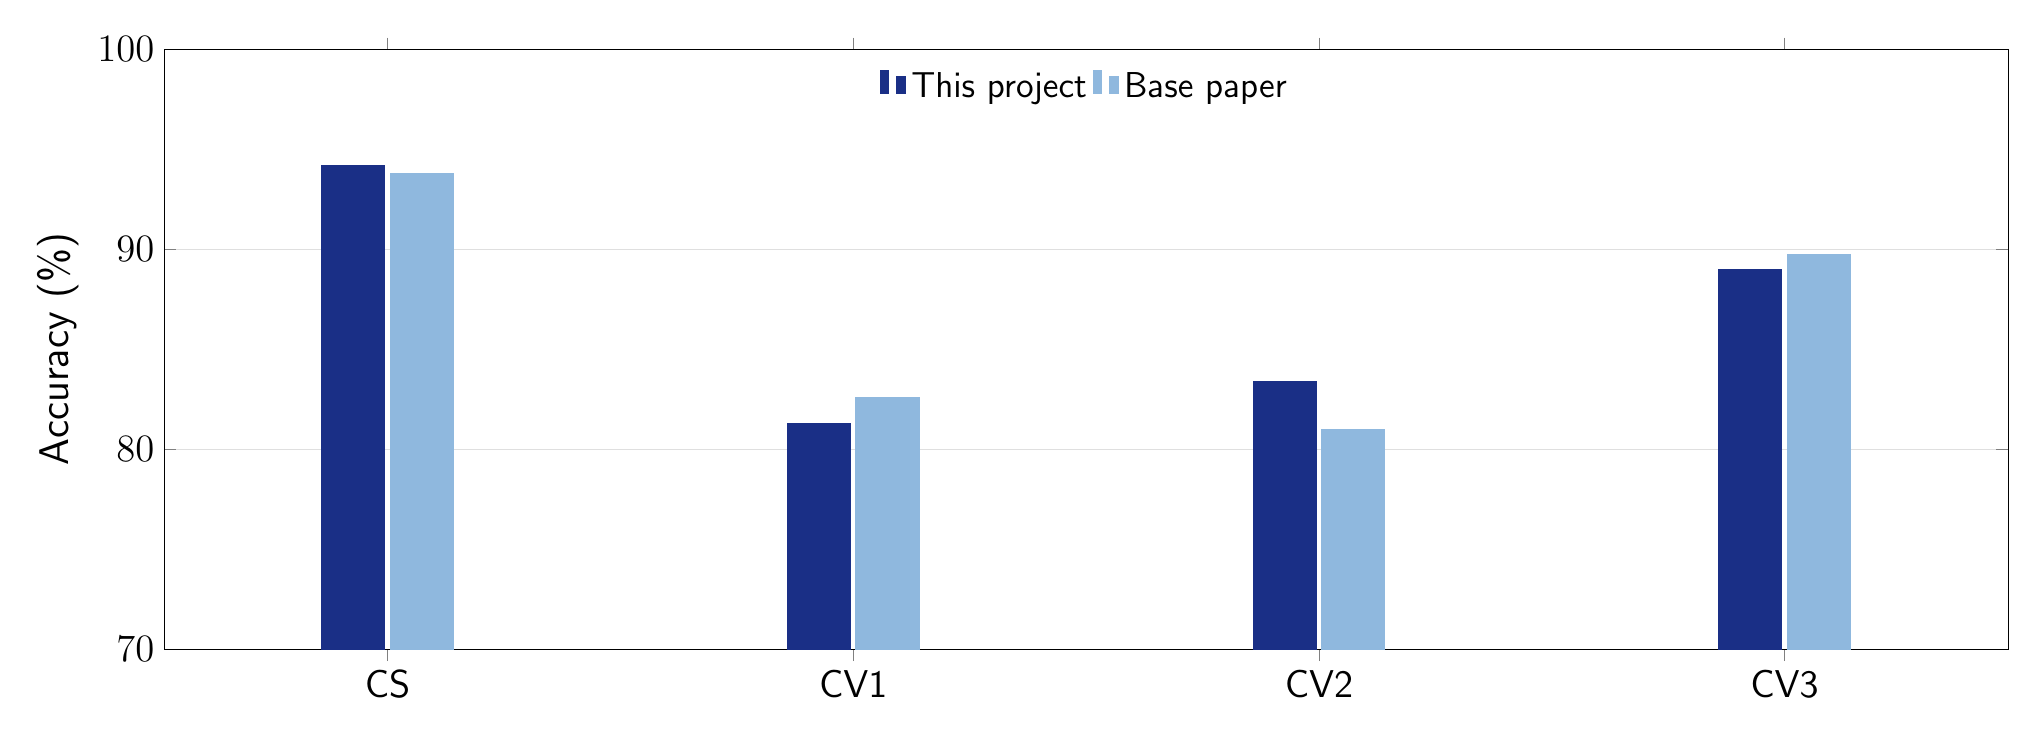
\begin{tikzpicture}
\begin{axis}[width=250mm,height=92mm,ybar,bar width=8mm,ymin=70,ymax=100,
  symbolic x coords={CS,CV1,CV2,CV3},xtick=data,
  ylabel={Accuracy (\%)},ytick={70,80,90,100},axis background/.style={fill=white},
  tick label style={font=\fontsize{14}{17}\selectfont},label style={font=\fontsize{15}{18}\selectfont},
  legend style={font=\fontsize{13}{16}\selectfont,at={(0.5,0.98)},anchor=north,legend columns=2,draw=none,fill=white},
  ymajorgrids,grid style={gray!25},enlarge x limits=0.16]
\addplot[fill=impc,draw=impc] coordinates {(CS,94.2) (CV1,81.3) (CV2,83.4) (CV3,88.97)};
\addplot[fill=refc,draw=refc] coordinates {(CS,93.81) (CV1,82.58) (CV2,81.00) (CV3,89.76)};
\legend{This project,Base paper}
\end{axis}
\end{tikzpicture}\\[1mm]
{\smalltext Fig.~2. Final accuracy against the base paper (CS: cross-subject; CV1--CV3: held-out camera).}
\end{minipage}\hfill
\begin{minipage}[t]{0.49\linewidth}\centering\vspace{0pt}
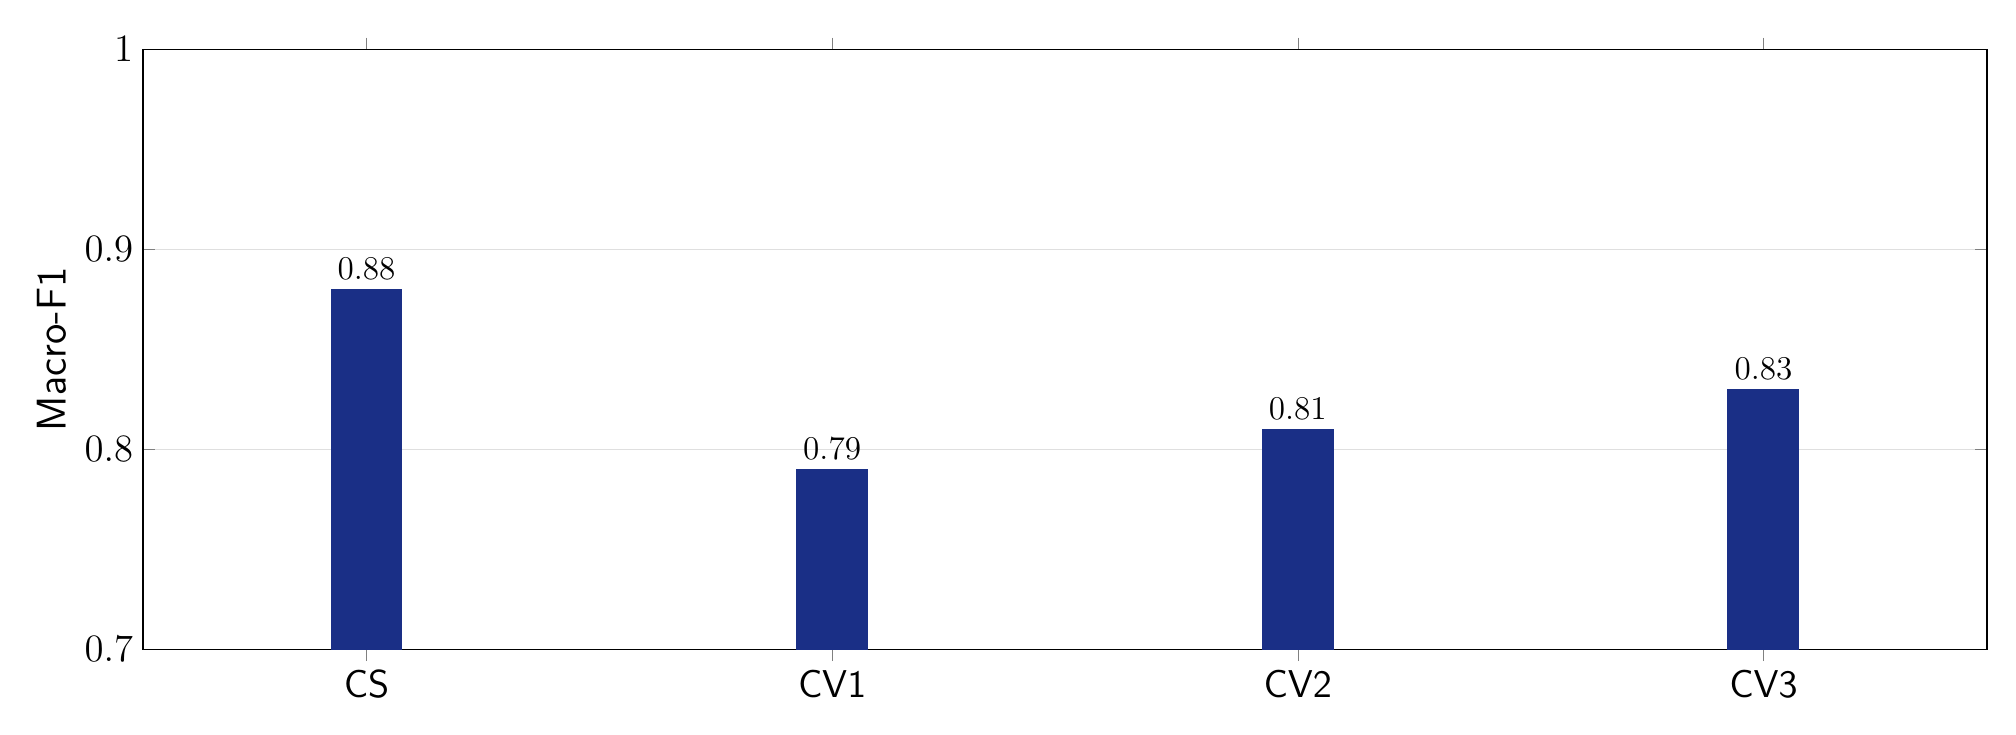
\begin{tikzpicture}
\begin{axis}[width=250mm,height=92mm,ybar,bar width=9mm,ymin=0.7,ymax=1.0,
  symbolic x coords={CS,CV1,CV2,CV3},xtick=data,
  ylabel={Macro-F1},ytick={0.7,0.8,0.9,1.0},axis background/.style={fill=white},
  tick label style={font=\fontsize{14}{17}\selectfont},label style={font=\fontsize{15}{18}\selectfont},
  ymajorgrids,grid style={gray!25},enlarge x limits=0.16,
  nodes near coords,nodes near coords style={font=\fontsize{12}{14}\selectfont}]
\addplot[fill=impc,draw=impc] coordinates {(CS,0.88) (CV1,0.79) (CV2,0.81) (CV3,0.83)};
\end{axis}
\end{tikzpicture}\\[1mm]
{\smalltext Fig.~3. Final macro-F1 on the same four protocols.}
\end{minipage}
\end{psec}

% ---------------- Conclusions | Translational Potential ----------------
\begin{tcbraster}[raster columns=2,raster equal height=rows,raster column skip=8mm,raster after skip=4mm]
\begin{psec}[after skip=0pt]{Conclusions}
\begin{itemize}
\item Built an end-to-end multi-view action recognition pipeline on NW-UCLA RGB~[3], from video grouping and segment sampling to evaluation and a demo.
\item Final cross-subject accuracy is 94.2\% (macro-F1 0.88), above the base paper's~[1] 93.81\%.
\item Final cross-view scores are 81.3\%, 83.4\% and 88.97\% onto cameras 1, 2 and 3 (macro-F1 0.79, 0.81 and 0.83).
\item Camera 3 remains 0.79 points below the base paper's 89.76\%. Next come per-component ablations and DVANet-style view supervision~[2].
\end{itemize}
\end{psec}
\begin{psec}[after skip=0pt]{Translational Potential}
\begin{itemize}
\item \textbf{Multi-camera surveillance:} recognizes actions from a camera position not used in training.
\item \textbf{Assisted living and healthcare:} monitoring daily activities such as sitting down, standing up and carrying.
\item \textbf{Lightweight:} a ResNet-18 backbone and a small Transformer train on a single GPU.
\item \textbf{No view labels:} the paired-view loss needs only synchronized clips, easing new camera setups.
\item \textbf{Ready demo:} classifies an input video and exports an annotated clip.
\end{itemize}
\end{psec}
\end{tcbraster}

% ---------------- Acknowledgements | References ----------------
\begin{tcbraster}[raster columns=2,raster equal height=rows,raster column skip=8mm,raster after skip=0mm,raster force size=false]
\begin{psec}[after skip=0pt,width=0.29\linewidth,fontupper=\smalltext]{Acknowledgements}
We thank the Image and Video Processing course instructor at IIIT Allahabad for guidance, the authors of the Northwestern-UCLA Multiview Action 3D dataset~[3], and Kaggle for GPU compute (NVIDIA Tesla T4).
\end{psec}
\begin{psec}[after skip=0pt,width=0.695\linewidth,fontupper=\fontsize{12}{14.2}\selectfont,top=3mm,bottom=3mm]{References}
\begin{enumerate}[label={[\arabic*]},leftmargin=2.1em,itemsep=0pt,topsep=0pt]
\item A.-V. Bui and T.-O. Nguyen, ``Multi-view human action recognition based on TSN architecture integrated with GRU,'' \textit{Procedia Comput. Sci.}, vol.~176, pp.~948--955, 2020.
\item N. Siddiqui, P. Tirupattur and M. Shah, ``DVANet: Disentangling view and action features for multi-view action recognition,'' in \textit{Proc. AAAI}, vol.~38, pp.~4873--4881, 2024.
\item J. Wang, X. Nie, Y. Xia, Y. Wu and S.-C. Zhu, ``Cross-view action modeling, learning and recognition,'' in \textit{Proc. IEEE CVPR}, 2014, pp.~2649--2656.
\item L. Wang \textit{et al.}, ``Temporal segment networks: Towards good practices for deep action recognition,'' in \textit{Proc. ECCV}, 2016, pp.~20--36.
\item K. Cho \textit{et al.}, ``Learning phrase representations using RNN encoder--decoder for statistical machine translation,'' in \textit{Proc. EMNLP}, 2014, pp.~1724--1734.
\item D. Wang, W. Ouyang, W. Li and D. Xu, ``Dividing and aggregating network for multi-view action recognition,'' in \textit{Proc. ECCV}, 2018, pp.~457--473.
\item H.-T. Nguyen and T.-O. Nguyen, ``Attention-based network for effective action recognition from multi-view video,'' \textit{Procedia Comput. Sci.}, vol.~192, pp.~971--980, 2021.
\item K. Shah, A. Shah, C. P. Lau, C. M. de Melo and R. Chellappa, ``Multi-view action recognition using contrastive learning,'' in \textit{Proc. IEEE/CVF WACV}, 2023, pp.~3381--3391.
\item C. Szegedy \textit{et al.}, ``Rethinking the Inception architecture for computer vision,'' in \textit{Proc. IEEE CVPR}, 2016, pp.~2818--2826.
\item K. He, X. Zhang, S. Ren and J. Sun, ``Deep residual learning for image recognition,'' in \textit{Proc. IEEE CVPR}, 2016, pp.~770--778.
\item A. Vaswani \textit{et al.}, ``Attention is all you need,'' in \textit{Proc. NeurIPS}, 2017, pp.~5998--6008.
\item I. Loshchilov and F. Hutter, ``Decoupled weight decay regularization,'' in \textit{Proc. ICLR}, 2019.
\item I. Loshchilov and F. Hutter, ``SGDR: Stochastic gradient descent with warm restarts,'' in \textit{Proc. ICLR}, 2017.
\item A. Paszke \textit{et al.}, ``PyTorch: An imperative style, high-performance deep learning library,'' in \textit{Proc. NeurIPS}, 2019, pp.~8024--8035.
\end{enumerate}
\end{psec}
\end{tcbraster}

\end{document}
